\documentclass[8pt,sans,aspectratio=1610]{beamer}
%aspectratio=32
%aspectratio=169
\usepackage{etex}
\usepackage{enumitem}
%\reserveinserts{28}
\usepackage{amssymb}
\usepackage{theorem}
%\usepackage{savetrees}
%\usepackage[landscape]{geometry}
%\usepackage[margin=2cm]{geometry}
\usepackage{graphicx}
\usepackage{fancybox}
\usepackage{fancyhdr}
\usepackage{tabularx}
\usepackage{color}
\usepackage{xcolor}
\usepackage{multirow}
\usepackage{amsmath}
\usepackage[utf8]{inputenc} % Pour pouvoir taper les accent directement et non pas passer par \'
\usepackage[T1]{fontenc} %%% Pour que les accents soient correctement traités dans le PDF et le DVI
\usepackage{lmodern} %Un autre package pour les accents français
\usepackage[french]{babel} %Un autre package pour les accents
\usepackage{ifthen}
%\usepackage{multicol}
%\usepackage{cancel}
\usepackage{pst-all}
\usepackage{pstricks-add}
\usepackage{multicol}
%\usepackage{tikz}
%\usepackage{pgf,tikz}
%\usepackage{circuitikz}
%\usetikzlibrary{shapes}
%\usetikzlibrary{calc}
%\usetikzlibrary{plotmarks}
%\usepackage{tkz-fct}
\usepackage{fp}
\usepackage{float}
%\usepackage{siunitx}
\usepackage{pdfpages}%Pour sortir seulement certaine pages du pdf
\usepackage{textcomp}
\usepackage{hyperref}
%\hypersetup{
%    colorlinks=true, % make the links colored
%    linkcolor=blue, % color TOC links in blue
%    urlcolor=red, % color URLs in red
%    linktoc=all % 'all' will create links for everything in the TOC
%}

%\sisetup{locale = FR, number-math-rm, per-mode=symbol, separate-uncertainty}
%\hypersetup{pdfpagemode=FullScreen}

\renewcommand{\exp}[1]{\mathrm{e}^{#1}}

%\setlength{\parindent}{0pt}


\begin{document}

\title{Les bandits stochastiques à récompenses d'espérance non-définie}
\author{Adam Cohen, Maxime Genest, Vincent Masse}
\maketitle

\begin{frame}
\frametitle{Rappel sur les bandits stochastiques classiques}
%\framesubtitle{Et son sous-titre}

\begin{itemize}

\item[$\bullet$] Ensemble de $K$ actions (bras, machines).

\item[$\bullet$] Chaque action $k$ est associée à un paramètre inconnu $\mu_k$ tel que $X_{k_t} \sim \nu\left(\mu_k\right)$ où $\nu\left(\mu_k\right)$ est une distribution d'espérance $\mu_k.$

\end{itemize}

\vfill

\pause

Dans le jeu des bandits stochastiques, à chaque pas de temps $t=1,2,\ldots,T,$ l'agent:

\begin{itemize}

\item[$\bullet$] Sélectionne une action $k_t\in\left\{1,2,\ldots K\right\}$ 

\item[$\bullet$] On observe une récompense (reward) $r_t\sim \nu\left(\mu_{k_t}\right).$

\end{itemize}

But: Déterminer une politique d'action qui maximisera $\displaystyle \mathbb{E}\left[\sum_{t=1}^T r_t\right]$\\

\vfill
\end{frame}


\begin{frame}
\frametitle{Mesure de performance empirique pour les bandits stochastiques}
Dans cette situation, à chaque pas de temps $t=1,2,\ldots,T,$ l'agent cumule un regret:

$$\Delta_{k_t}=\mu^{\star}-\mu_{k_t}$$ 
 
À la fin de l'épisode, on peut calculer le regret cumulatif empirique:

$$R(T)=\sum_{t=1}^T \Delta_{k_t}$$

Cela nous permet de comparer empiriquement la performance de plusieurs politiques, en simulant plusieurs épisodes et en comparant le regret cumulatif moyen sur ces épisodes.  

\end{frame}

\begin{frame}
\frametitle{L'hypothèse d'existence de l'espérance}
Le jeu des bandits stochastiques ainsi présenté sous-entend que la distribution des rewards associés aux bras du bandit est d'espérance qui existe. Or, plusieurs lois de probabilité ont une \textbf{espérance non-définie}. 

\pause
\vfill

Par exemple, la loi de Cauchy ou certaines configuration de la loi de Pareto.

\pause
\vfill

\textbf{Intérêts du projet}


\begin{itemize}
\item[$\bullet$]
Intérêt personnel (curiosité intellectuel).

\pause
\vfill

\item[$\bullet$]
Modélisation du temps d'attente/temps de service par des distributions à queues lourdes.

\pause
\vfill

{\it Yu Li. Queuing theory with heavy tails and network traffic modeling. 2018. hal-01891760}

\vfill

{\it Whitt, Ward. (2000). The impact of a heavy-tailed service-time distribution upon the M/GI/s waiting-time distribution. Queueing Syst.. 36. 71-87. 10.1023/A:1019143505968.}

\end{itemize}

\vfill

\end{frame}

%\begin{frame}
%\frametitle{La loi de Cauchy}
%La loi de Cauchy est une loi continue de fonction de densité 
%
%$$f(x;L;a)=\frac{1}{\pi\,a\left[1+\left(\frac{x-L}{a}\right)^2\right]}=\frac{1}{\pi}\left[\frac{a}{(x-L)^2+a^2}\right]$$
%
%où $L\in\mathbb{R}$ est un paramètre de localisation et $a>0$ est un paramètre d'échelle.
%
%\pause
%
%\begin{figure}[H]
%\begin{center}
%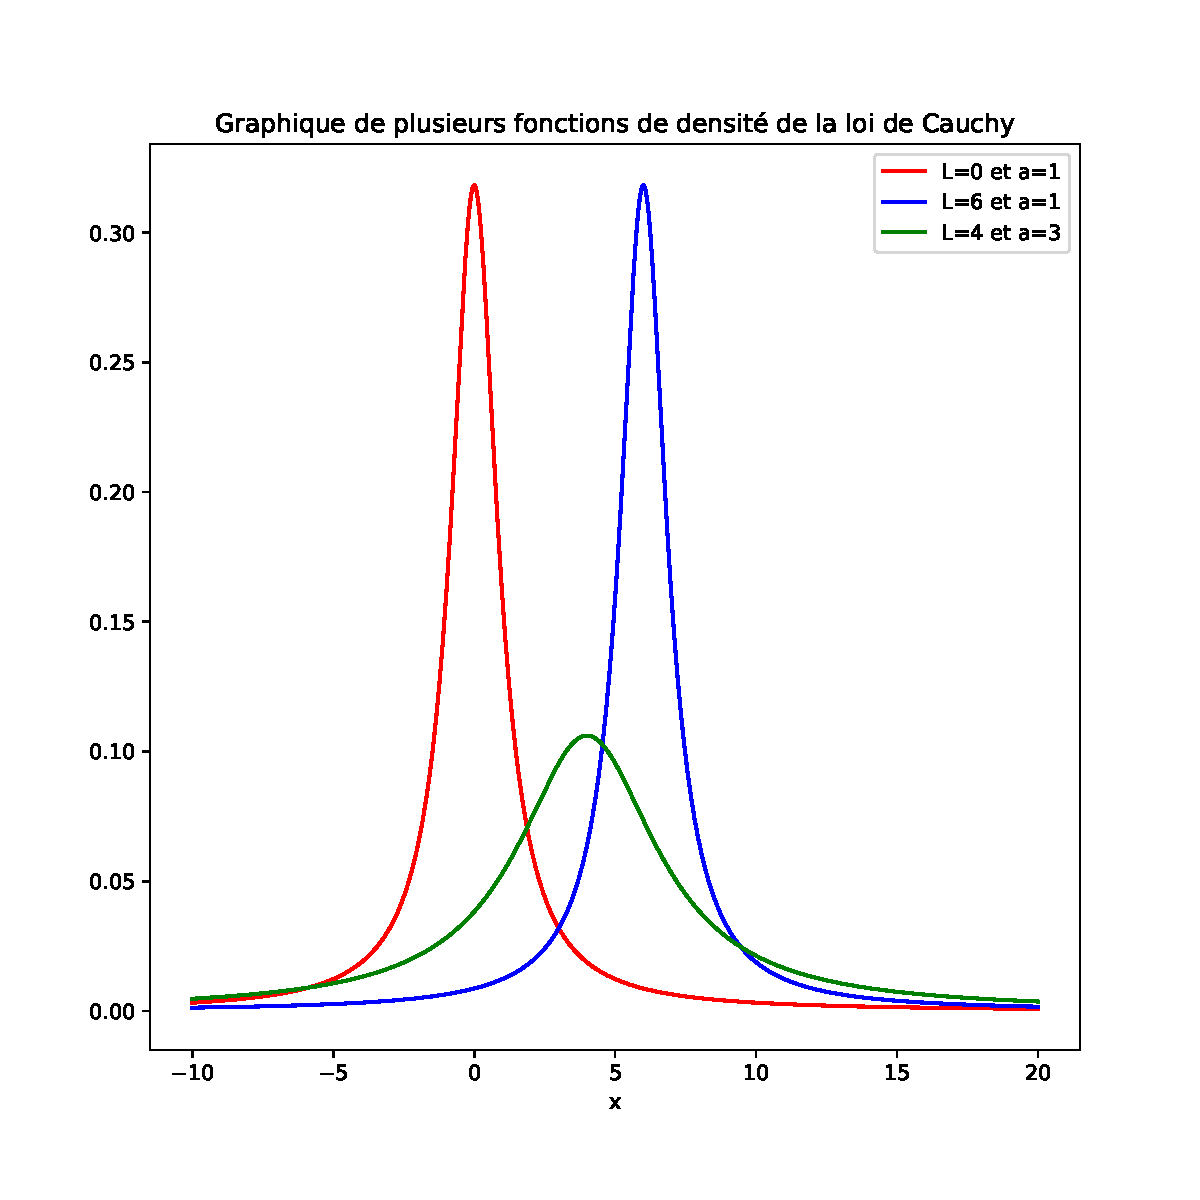
\includegraphics[scale=0.3]{graphiques_Cauchy.pdf}
%\end{center}
%\end{figure}
%
%\end{frame}

\begin{frame}
\frametitle{La loi de Cauchy}
La loi de Cauchy est une loi continue de fonction de densité 

$$f(x;L;a)=\frac{1}{\pi\,a\left[1+\left(\frac{x-L}{a}\right)^2\right]}=\frac{1}{\pi}\left[\frac{a}{(x-L)^2+a^2}\right]$$

où $L\in\mathbb{R}$ est un paramètre de localisation et $a>0$ est un paramètre d'échelle.

\pause
\vspace*{-0.5cm}

\begin{columns}[T]

\begin{column}{0.5\linewidth}

\begin{center}
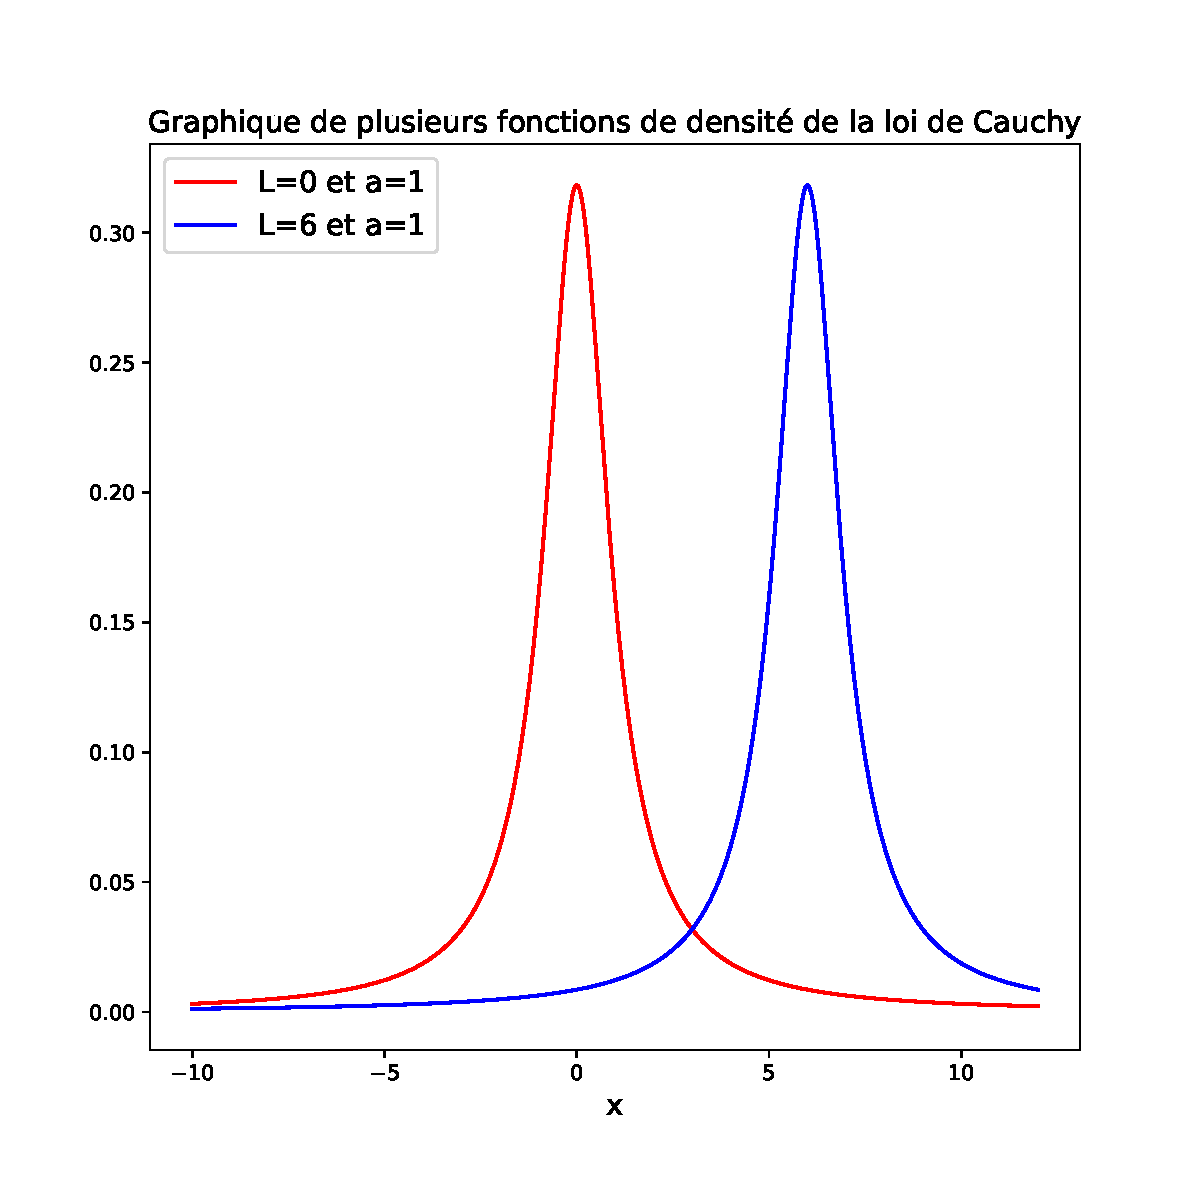
\includegraphics[scale=0.3]{graphiques_Cauchy-2.pdf}
\end{center}

\end{column}

\pause

\begin{column}{0.5\linewidth}

\vspace*{3cm}

Soit $X\sim\mathrm{Cauchy}(0,1)$ et $Y\sim\mathrm{Cauchy}(6,1),$ alors $\forall t\in\mathbb{R},~\mathbb{P}[Y>t]>\mathbb{P}[X>t]$

\end{column}

\end{columns}

\end{frame}


\begin{frame}

\frametitle{Les bandits de Cauchy}

À chaque pas de temps $t=1,2,\ldots,T,$ l'agent:

\begin{itemize}

\item[$\bullet$] Sélectionne une action $k_t\in\left\{1,2,\ldots,K\right\}$

\item[$\bullet$] Observe une reward $r_t\sim \mathrm{Cauchy}(L_{k_t},a)$

\end{itemize}

\vfill
\pause

L'action optimale et la localisation optimale sont définis à partir de la localisation des différents bras:

\pause
$$\displaystyle L^{\star} := \max_k L_k \qquad \text{et} \qquad k^{\star} := \underset{k}{\mathrm{argmax}} L_k$$ 

\pause
\vfill

le gap (regret) associé à l'action $k$ devient $\Delta_k= L^{\star}-L_k$ 

\pause
\vfill

Mesure de performance empirique d'un agent: $\displaystyle R(T)=\sum_{t=1}^T \Delta_{k_t}$

\end{frame}

\begin{frame}
\frametitle{Les algorithmes classiques : Exemple d'échec}

\textbf{Expérience}\\
Pour chacune des $N=200$ répétitions,\\

\begin{itemize}

\item[$\bullet$] Créer un bandit Cauchy à deux bras de distributions $\mathrm{Cauchy}(5,1)$ et $\mathrm{Cauhy}(6,1).$

\item[$\bullet$] Jouer $\epsilon$-greedy et $\epsilon_t$-greedy sur un horizon de $T=1000$ pas de temps. 
\end{itemize}

Tracer le regret cumulatif empirique moyenné sur les $N$ répétitions.

\vfill
\pause

\begin{columns}[T] % align columns
\begin{column}{0.5\linewidth}

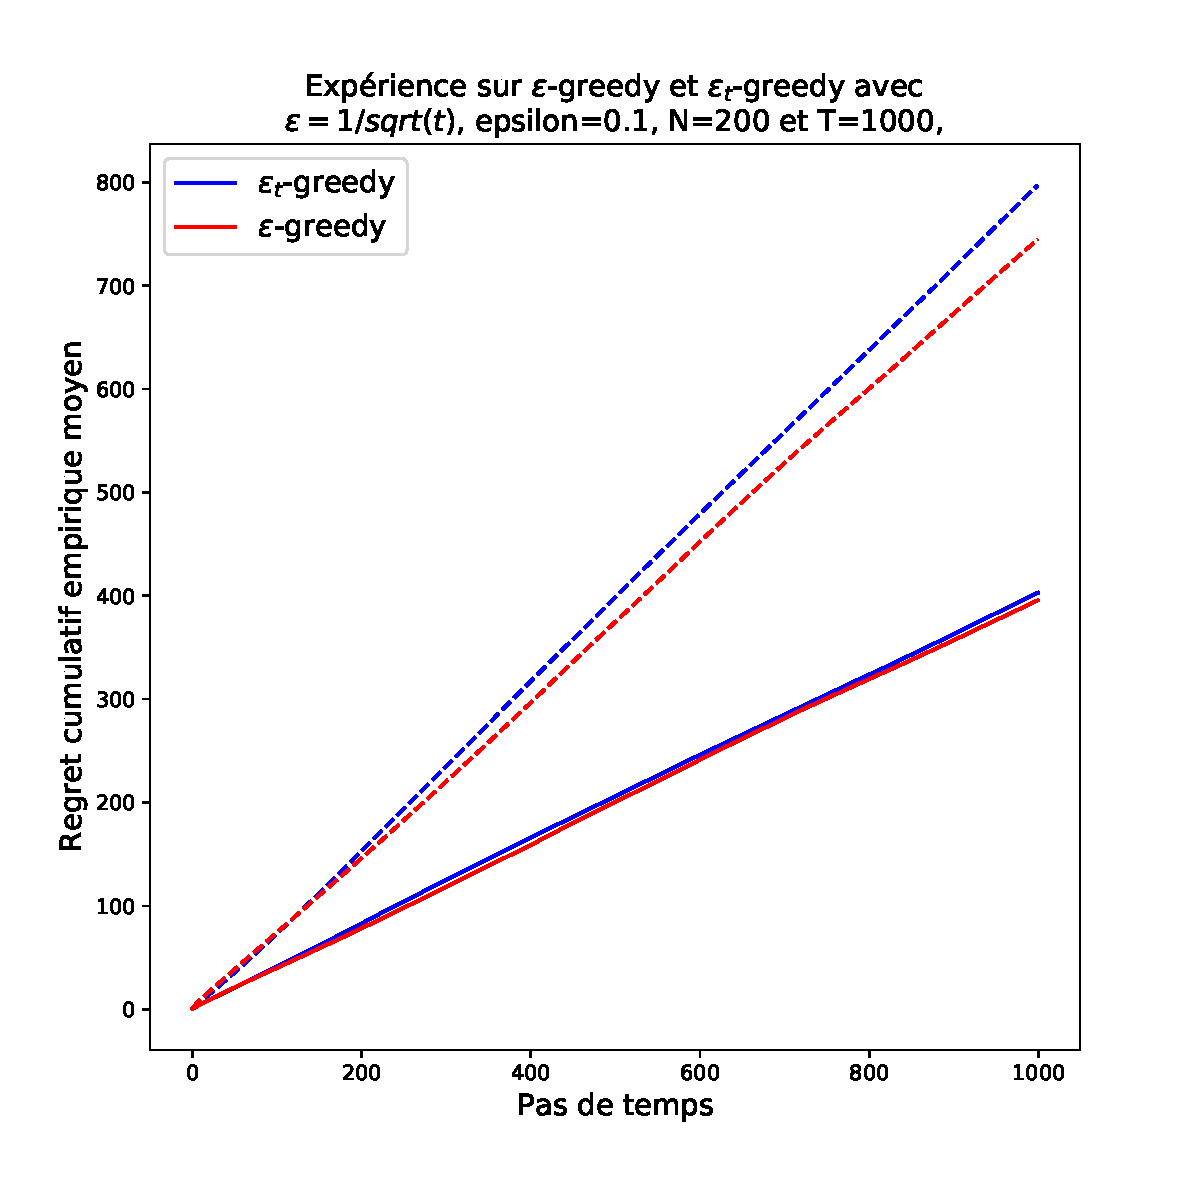
\includegraphics[scale=0.3]{contre-exemple-epsilon-greedy.pdf}

\end{column}
\pause
\begin{column}{0.5\linewidth}

\vspace*{1cm}
Cause de la mauvaise performance: $\epsilon$-greedy base le choix de son action d'exploitation sur la moyenne empirique $\hat \mu_k(t)$ des rewards reçus en jouant \mbox{l'action $k.$}

\vspace*{1cm}
\pause
Cet estimateur (la moyenne empirique) n'estime pas bien la localisation $L_k$ du bras numéro $k.$

\vfill
\end{column}
\end{columns}

\end{frame}

\begin{frame}
\frametitle{La non-convergence de la moyenne empirique}

Comportement de la moyenne empirique sur une séquence de réalisations provenant d'une loi $\mathrm{Cauchy}(5,1)$

\pause

\begin{columns}[T] % align columns
\begin{column}{0.5\linewidth}
%\color{red}\rule{\linewidth}{4pt}
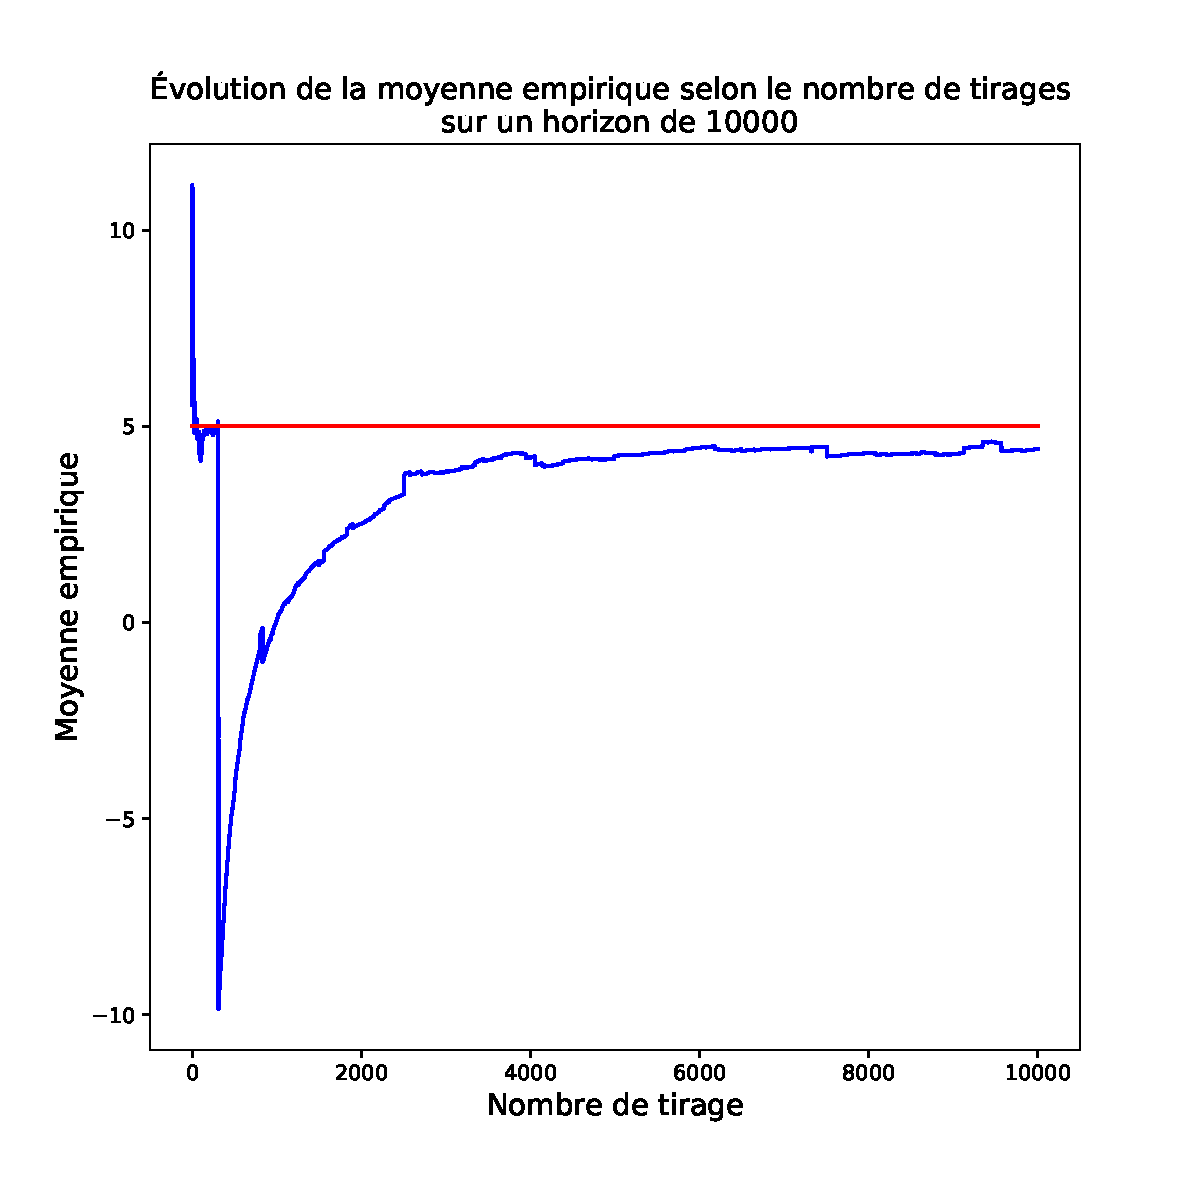
\includegraphics[scale=0.28]{graphique-moyenne-empirique-1.pdf}
\end{column}%
\hfill%

\pause

\begin{column}{0.5\linewidth}
%\color{blue}\rule{\linewidth}{4pt}
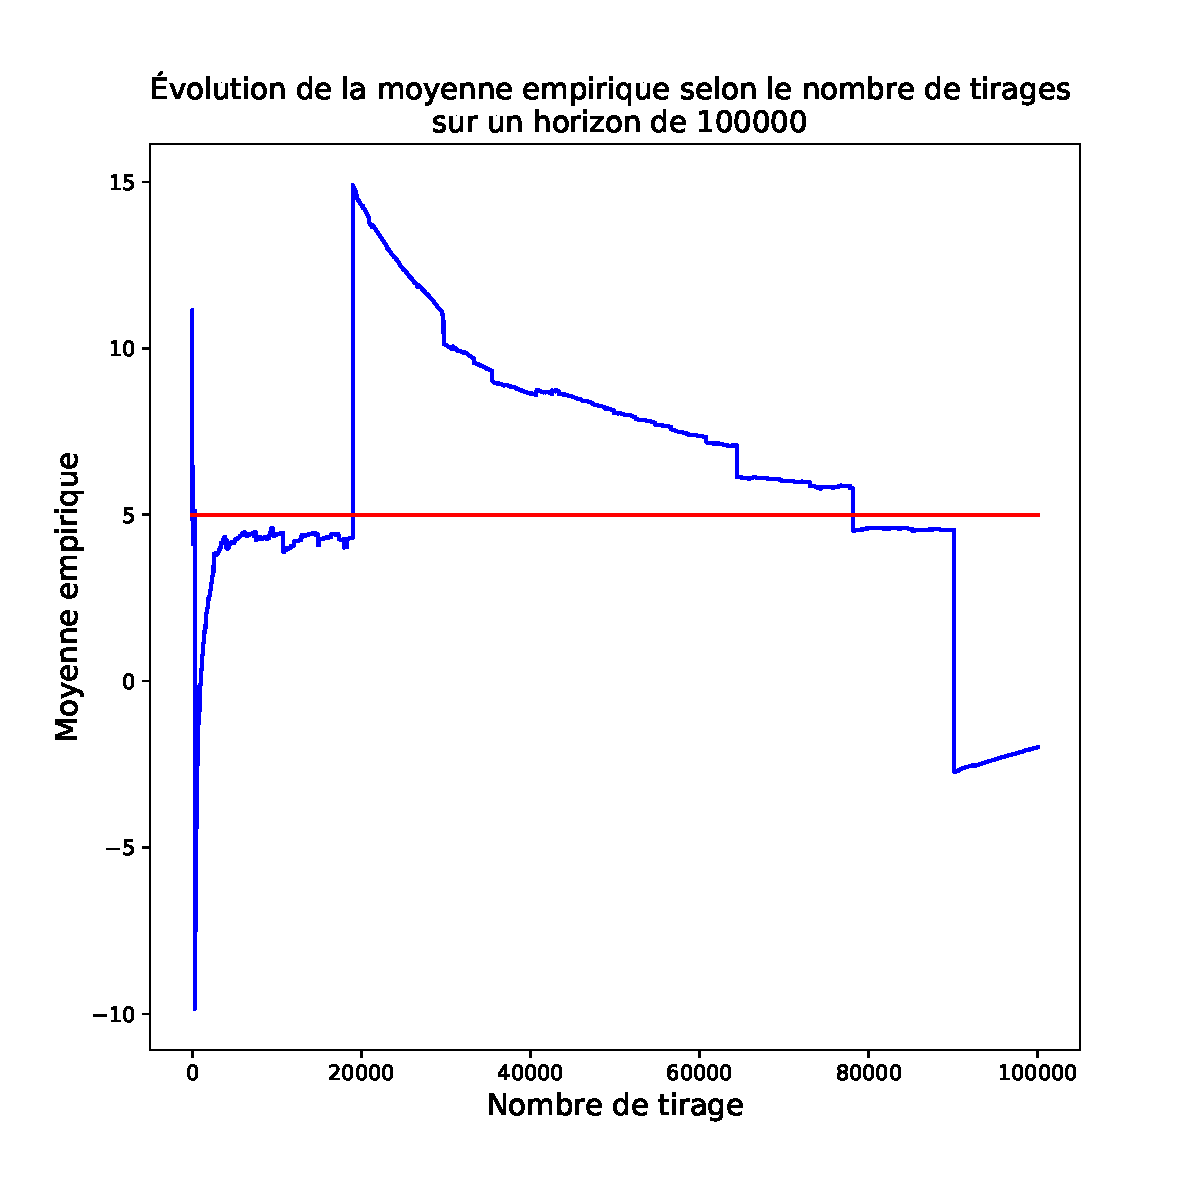
\includegraphics[scale=0.28]{graphique-moyenne-empirique-2.pdf}
\end{column}%
\end{columns}

\end{frame}


\begin{frame}

\frametitle{Estimateurs de localisation d'une loi de Cauchy}

Soit $\mathcal{X}=\left\{X_1,X_2,...,X_T\right\}$ une séquence d'observations provenant d'une loi $\mathrm{Cauchy}(L,a)$ où $L$ est inconnu et $a$ connu.

\vfill
\pause

\begin{itemize}
%\item[$\bullet$]
%La moyenne empirique: $\displaystyle\overline{x}=\frac{1}{T}\sum_{i=1}^T X_i$

\vfill
\item[$\bullet$]
La médiane empirique: $\mathrm{MED}(\mathcal{X})$

\pause
\vfill
\item[$\bullet$]
La moyenne $\alpha-$tronquée: $\displaystyle TM_{\alpha}(\mathcal X)=\frac{1}{T-2r}\sum_{i=r+1}^{T-r}X_{(i)},$ où $X_{(i)}$ est la $i^\text{ième}$ statistique d'ordre de $\mathcal{X}.$

où $r=\left\lfloor n\alpha\right\rfloor$ où $0<\alpha<0.5$ 

\pause
\vfill
\item[$\bullet$]
L'estimateur de maximum de vraisemblance: $\mathrm{MLE}(\mathcal{X})$

\pause
\vfill
\item[$\bullet$]
L-estimator: $\displaystyle\mathrm{LE}(\mathcal{X})=\frac{1}{T}\sum_{i=1}^T J\left(\frac{i}{T+1}\right) X_{(i)}$, où $X_{(i)}$ est la $i^\text{ième}$ statistique d'ordre de $\mathcal{X},$\\

et $J(u)=\frac{\sin\left(4\pi(u-0.5\right)}{\tan\left(\pi(u-0.5\right)},$ 
\end{itemize}

\pause
\vfill

{\it Zhang, J. A highly efficient L-estimator for the location parameter of the Cauchy distribution. Comput Stat 25, 97–105 (2010)}

\end{frame}

\begin{frame}
\frametitle{Comportement des estimateurs de localisation de la loi de Cauchy }
%\framesubtitle{Les moyennes tronquées}
Comportement des moyennes tronquées sur une séquence de réalisations provenant d'une loi $\mathrm{Cauchy}(5,1)$

\pause

\begin{columns}[T] % align columns

\begin{column}{0.5\linewidth}

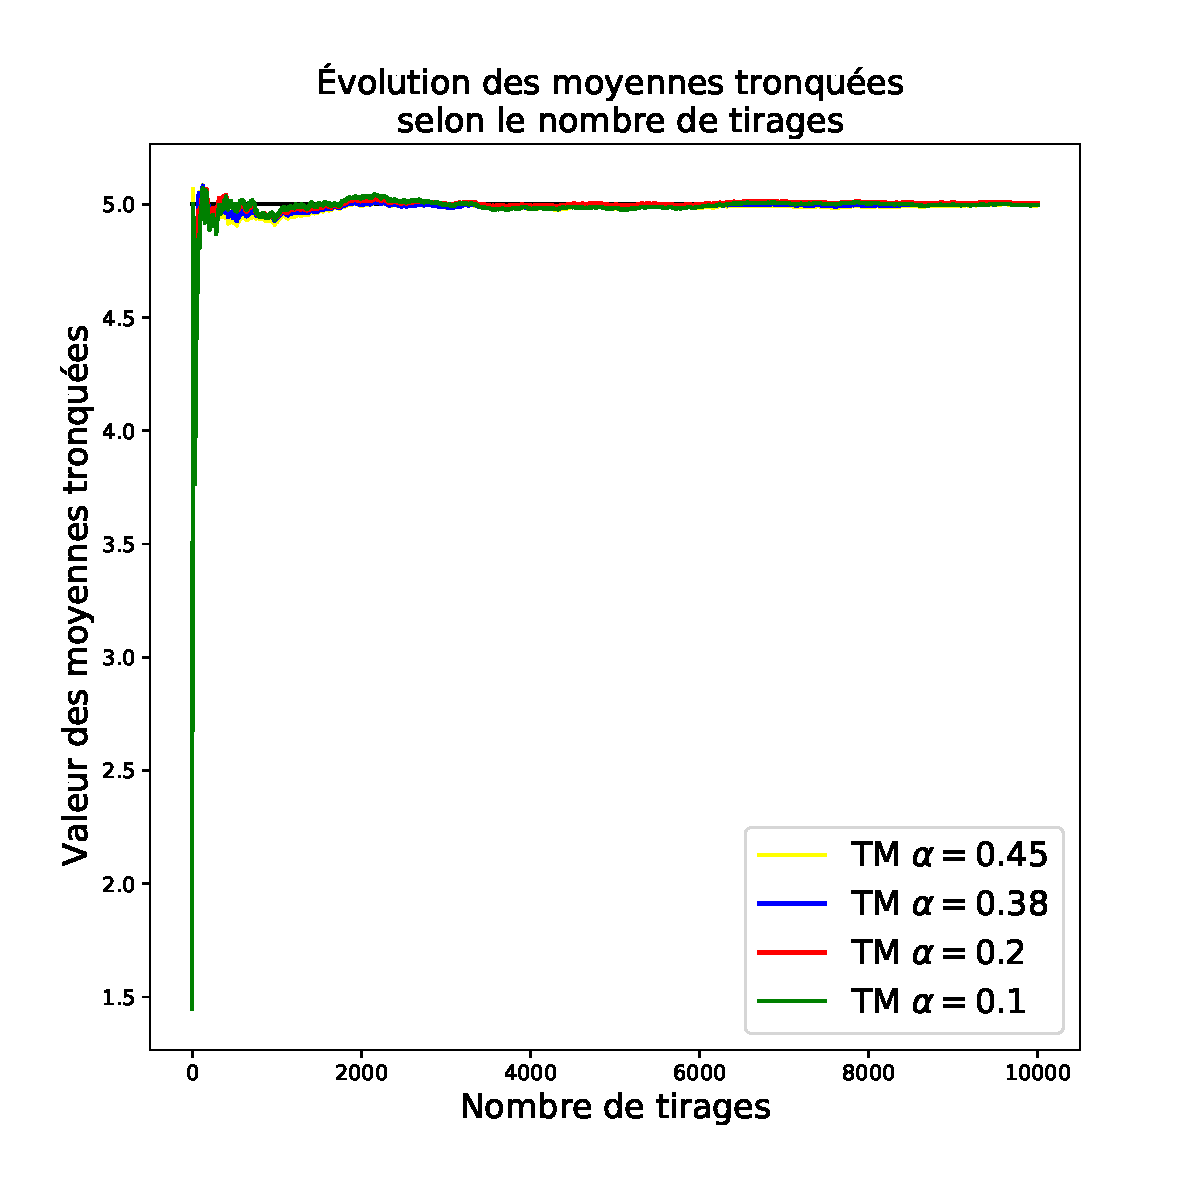
\includegraphics[scale=0.3]{mt-10000.pdf}

\end{column}

\pause
\hfill

\begin{column}{0.5\linewidth}

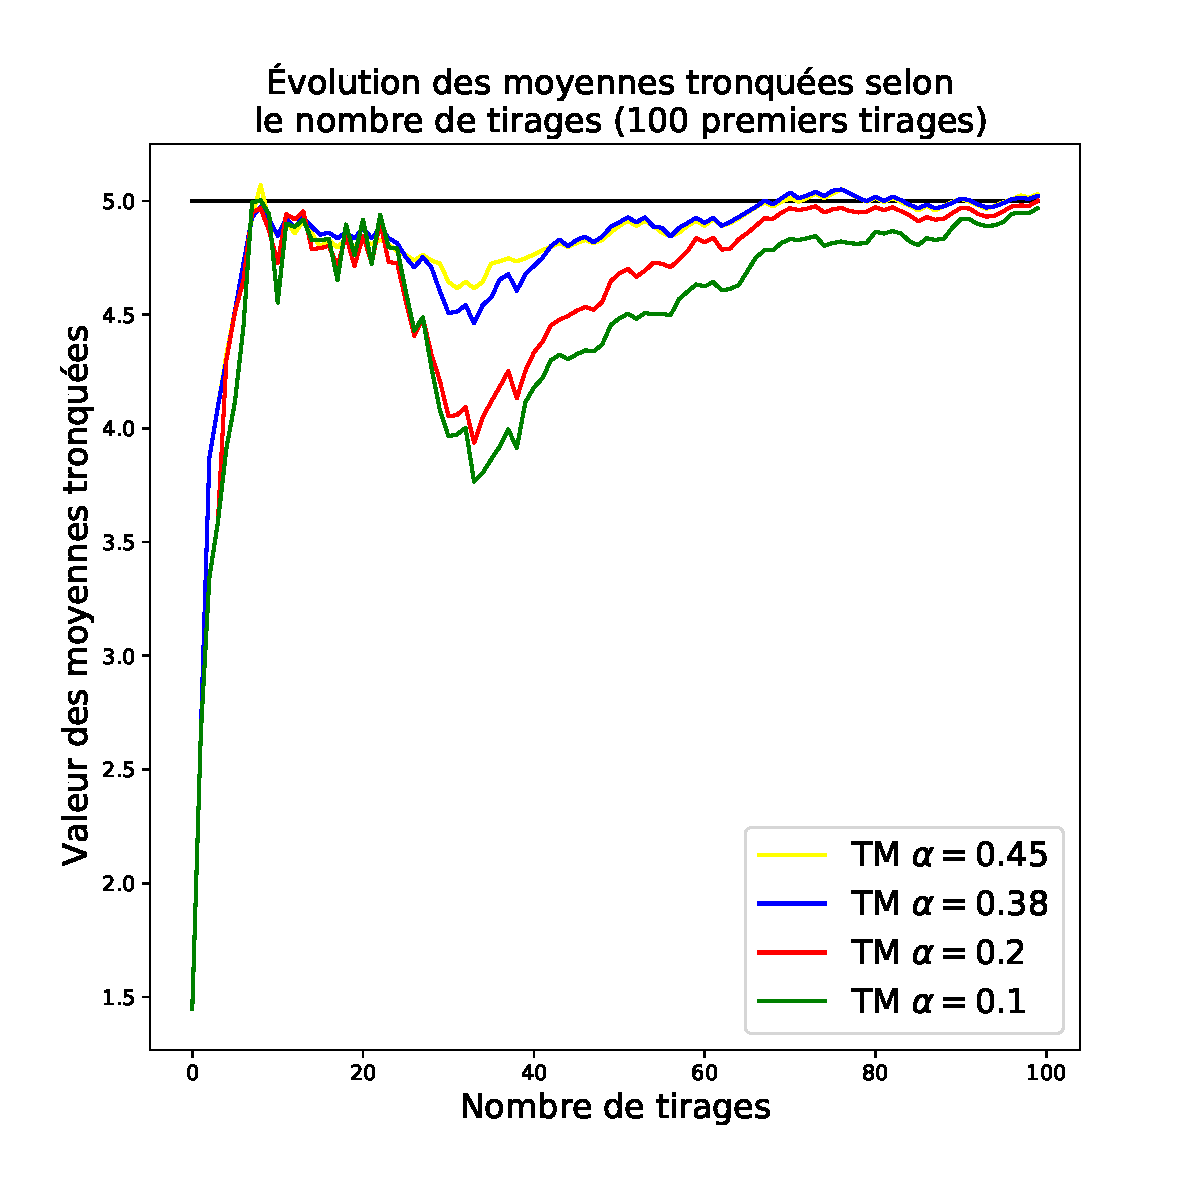
\includegraphics[scale=0.3]{mt-100.pdf}

\end{column}

\end{columns}

\vfill


\end{frame}

\begin{frame}

\frametitle{Comportement des estimateurs de localisation de la loi de Cauchy }
%\framesubtitle{Les moyennes tronquées}
Comportement des estimateurs ME, MLE, LE sur une séquence de réalisations provenant d'une loi $\mathrm{Cauchy}(5,1)$

\pause

\begin{columns}[T] % align columns

\begin{column}{0.5\linewidth}

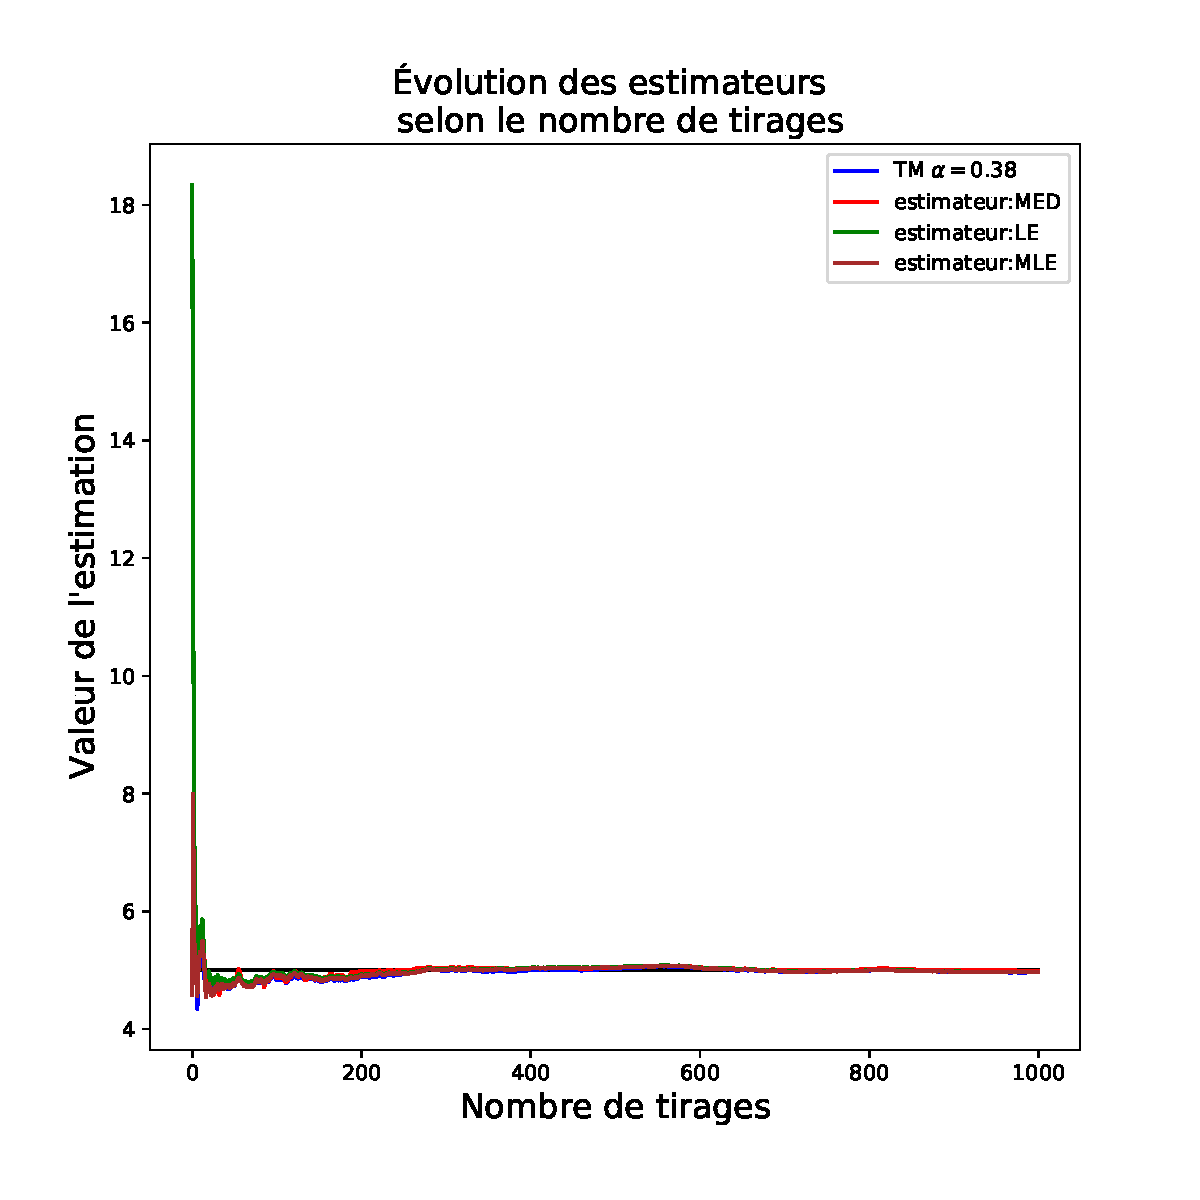
\includegraphics[scale=0.3]{Est-1000.pdf}

\end{column}

\pause
\hfill

\begin{column}{0.5\linewidth}

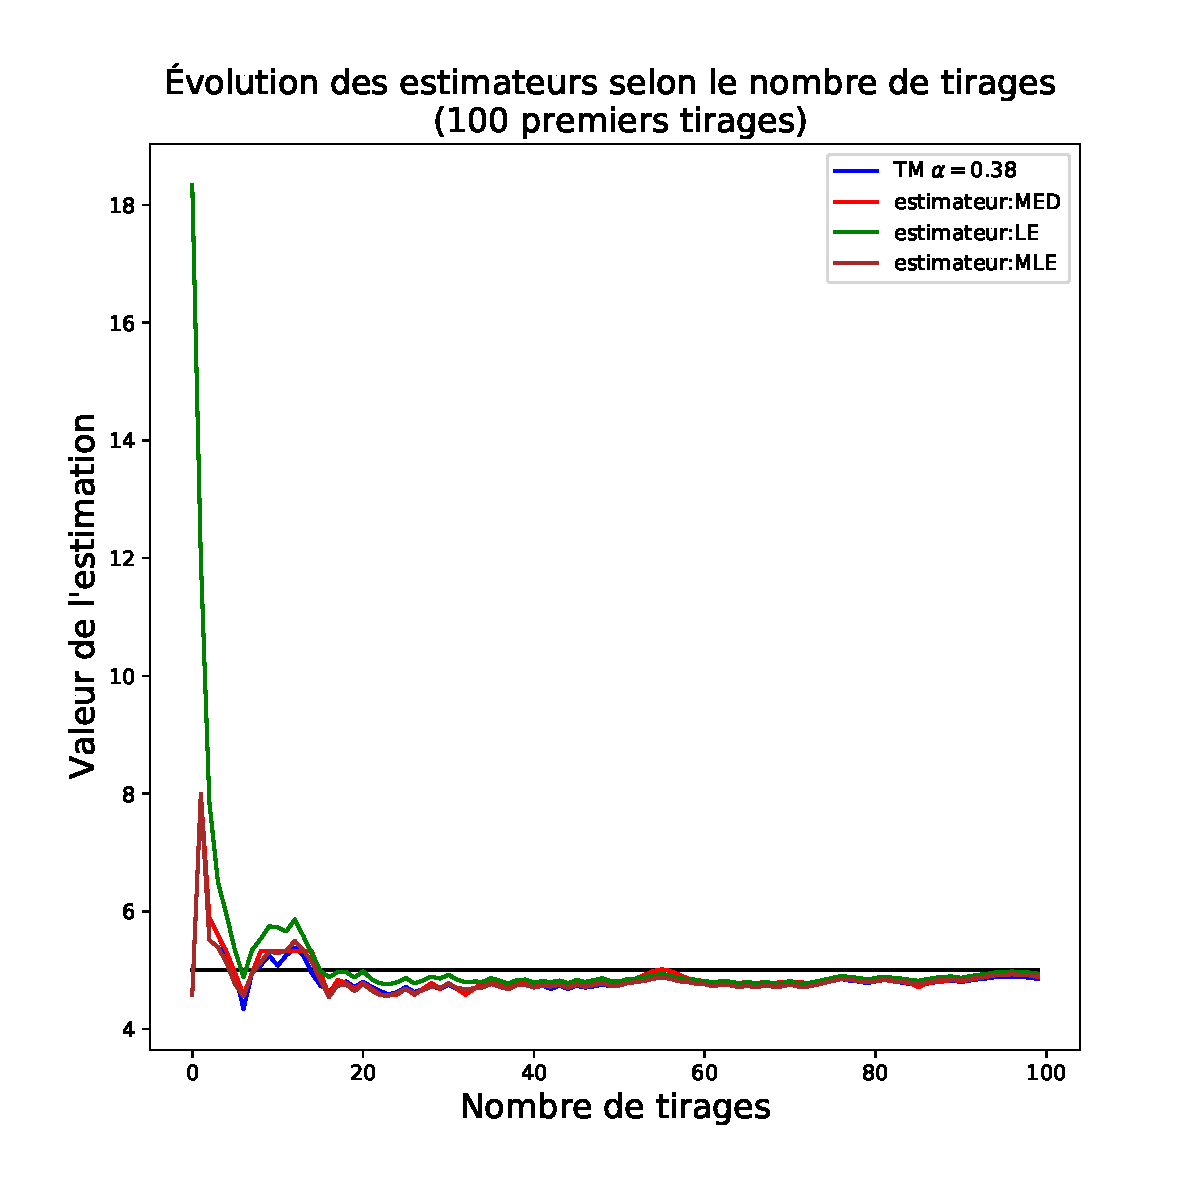
\includegraphics[scale=0.3]{Est-100.pdf}

\end{column}

\end{columns}

\vfill


\end{frame}


\begin{frame}
\frametitle{Adaptation des algorithmes existants}
\pause

\textbf{Exemple: adaptation de $\epsilon$-greedy}

\vfill
\pause

\underline{$\epsilon$-greedy classique}\\

\vfill
\pause

Pour tout $t\geq 1:$

\begin{itemize}
\item[$\bullet$] Explorer avec probabilité $\epsilon:$ Sélectionner $k_t\sim\mathcal{U}({1,2,...,K}).$
\item[$\bullet$] Exploiter avec probabilité $1-\epsilon:$ Sélectionner $k_t=\underset{k}{\mathrm{argmax}}\, \hat{\mu}_k(t-1)$
\end{itemize}

\pause
\vfill

\underline{$\epsilon$-greedy Cauchy}

\pause
\vfill
Pour tout $t\geq 1:$

\begin{itemize}
\item[$\bullet$] Explorer avec probabilité $\epsilon:$ Sélectionner $k_t\sim\mathcal{U}({1,2,...,K}).$
\item[$\bullet$] Exploiter avec probabilité $1-\epsilon:$ Sélectionner $k_t=\underset{k}{\mathrm{argmax}}\, \widehat{L_k}(t-1)$
\end{itemize}

\vfill

où $\widehat{L_k}(t-1)$ est un des estimateurs de la localisation $L_k$ du bras no $k$ basée sur les observations obtenus sur ce bras dans les pas de temps passés.

\pause
\vfill

De la même façon, on peut adapter aisément les $\underline{\epsilon_t\text{-greedy}}$,
$\underline{\text{ETC}}$ et $\underline{\text{Boltzmann/Softmax}}$ 

\end{frame}

\begin{frame}

\frametitle{Expérience 1 avec $\epsilon_t$-greedy avec $\epsilon_t=1/\sqrt{t}$ sur des bandits Cauchy}

\pause

Pour chacune des $N=200$ répétitions,\\

\pause

\begin{itemize}

\item[$\bullet$] Créer un bandit Cauchy à deux bras de distributions $\mathrm{Cauchy}(5,1)$ et $\mathrm{Cauhy}(6,1).$

\pause
\item[$\bullet$] Jouer $\epsilon_t$-greedy sur un horizon de $T=1000$ pas de temps (refaire avec plusieurs estimateurs de localisation pour adapter $\epsilon_t$-greedy)
\end{itemize}

\pause

Tracer le regret cumulatif empirique moyenné sur les $N$ répétitions pour comparer les différentes versions de l'algorithme.

\pause
\vspace*{-0.5cm}

\begin{columns}[T]

\begin{column}{0.5\linewidth}

\begin{center}
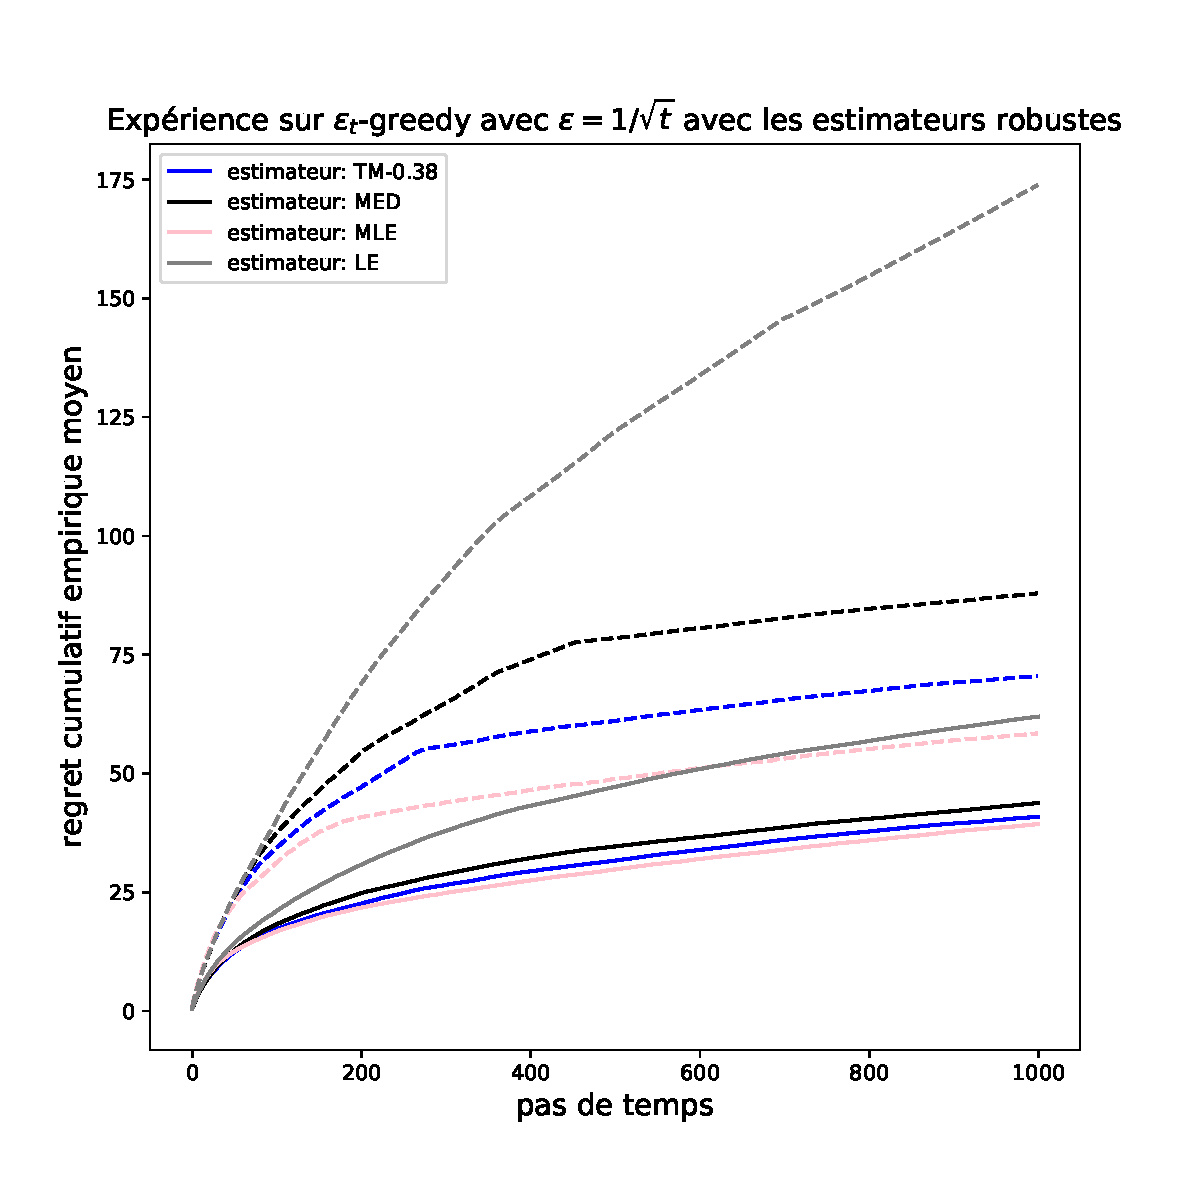
\includegraphics[scale=0.3]{experience-epsilon-t-greedy.pdf}
\end{center}

\end{column}

\pause
\hfill

\begin{column}{0.5\linewidth}

\begin{center}
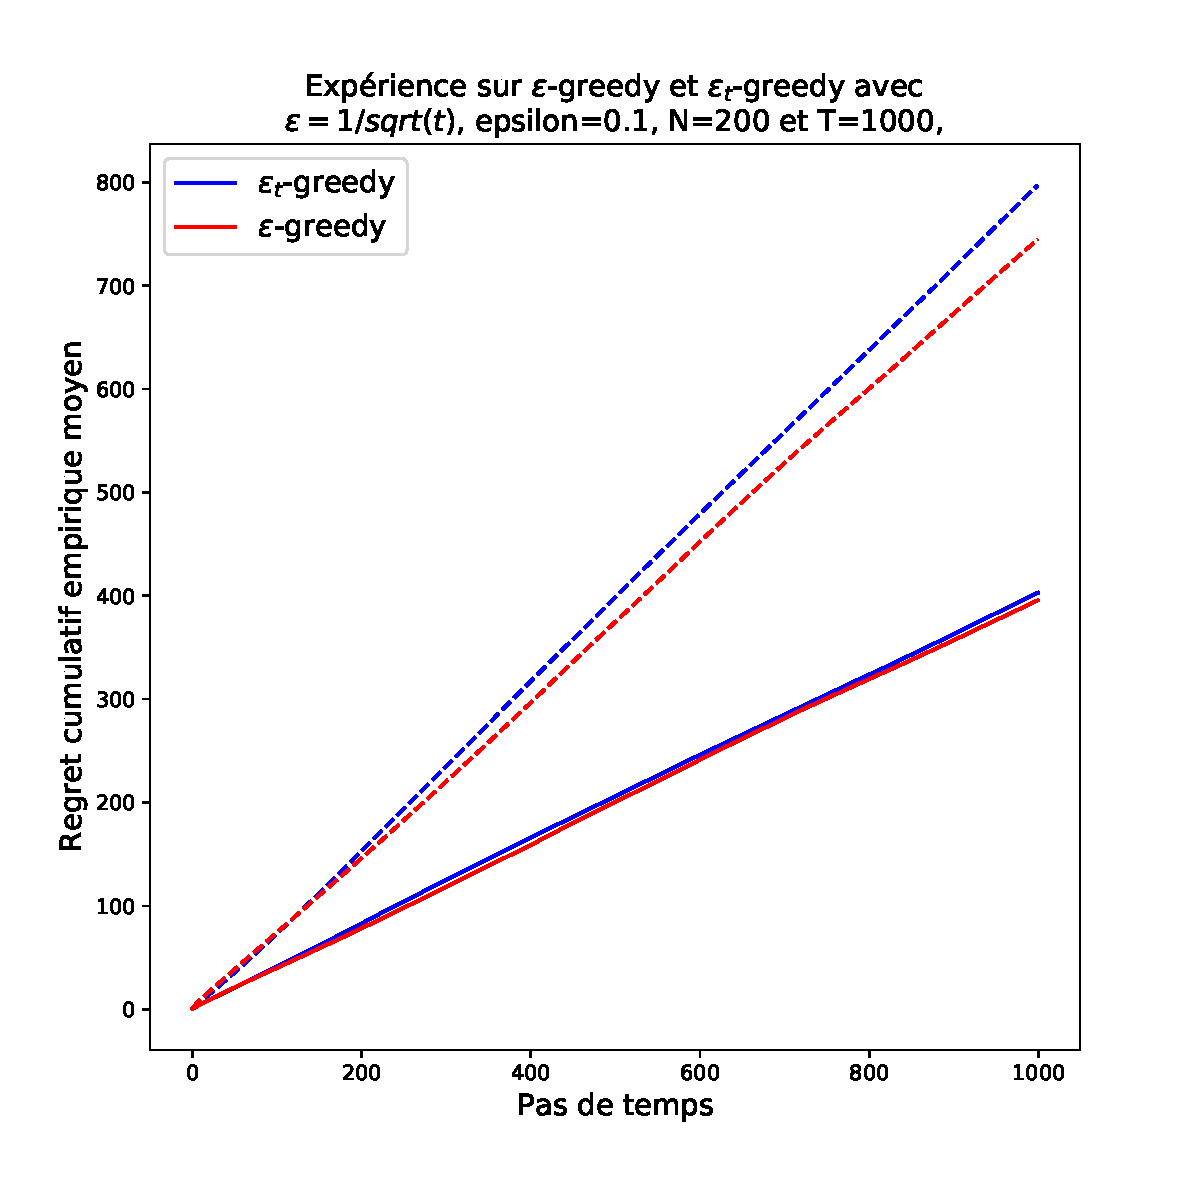
\includegraphics[scale=0.3]{contre-exemple-epsilon-greedy.pdf}
\end{center}

\end{column}

\end{columns}

\end{frame}

\begin{frame}

\frametitle{Expérience 2 avec $\epsilon_t$-greedy avec $\epsilon_t=1/\sqrt{t}$ sur des bandits Cauchy}

Pour chacune des $N=200$ répétitions,\\

\begin{itemize}

\item[$\bullet$] Créer un bandit Cauchy à deux bras de distributions $\mathrm{Cauchy}(L_1,1)$ et $\mathrm{Cauhy}(L_2,1)$ avec $L_1,L_2\sim\mathcal{U}([0,5])$

\item[$\bullet$] Jouer $\epsilon_t$-greedy sur un horizon de $T=1000$ pas de temps (refaire avec plusieurs estimateurs de localisation pour adapter $\epsilon_t$-greedy)
\end{itemize}

Tracer le regret cumulatif empirique moyenné sur les $N$ répétitions pour comparer les différentes versions de l'algorithme.

\begin{center}
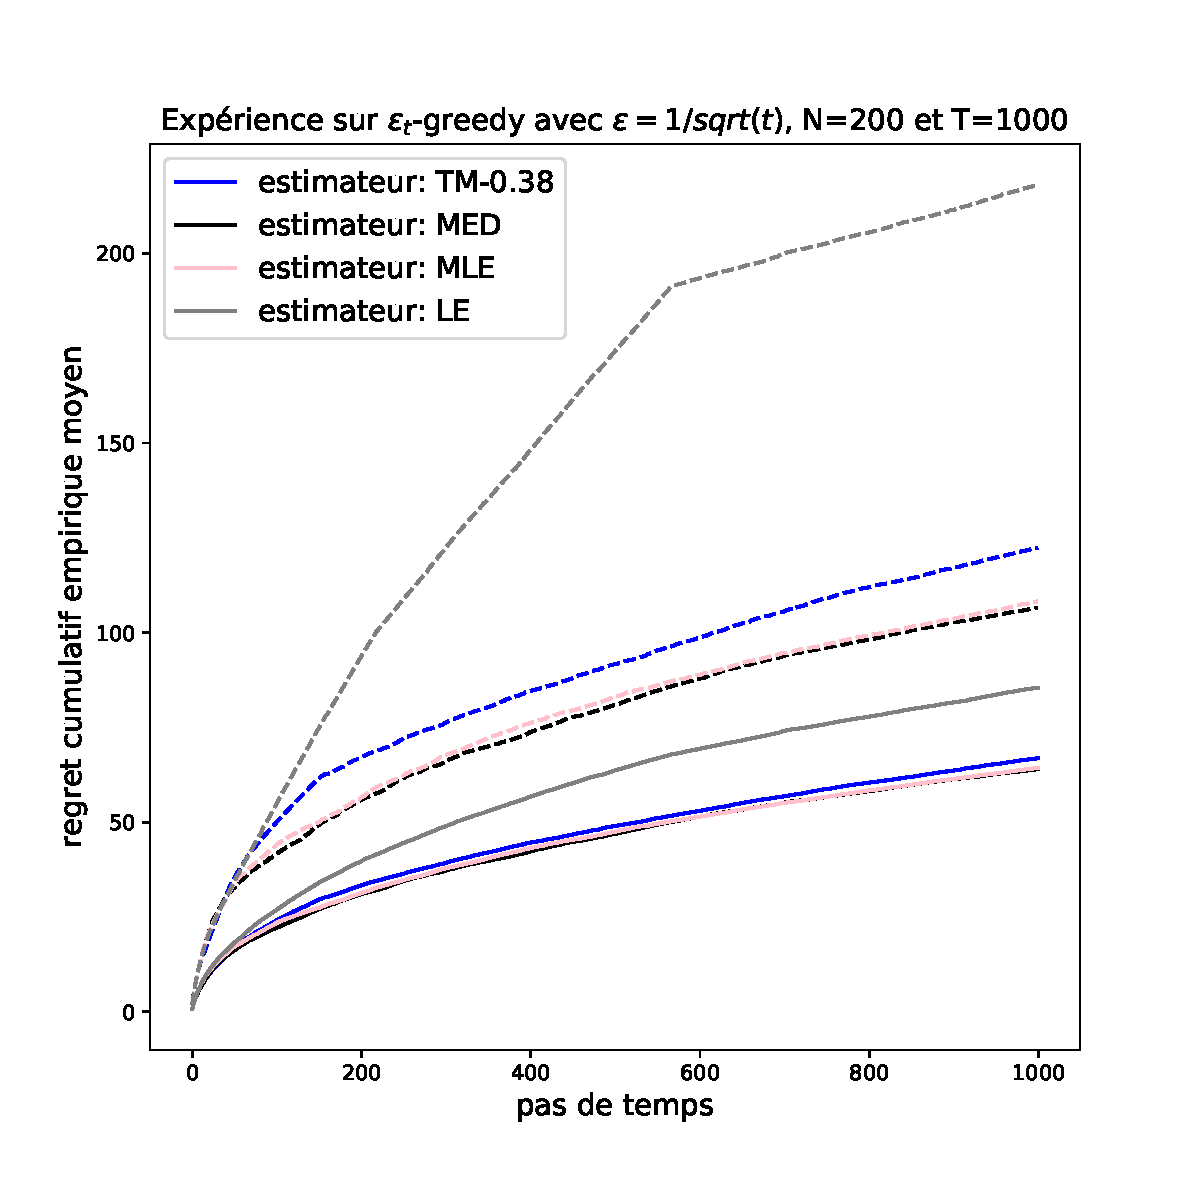
\includegraphics[scale=0.3]{experience-epsilon-t-greedy-2.pdf}
\end{center}

\end{frame}


\begin{frame}
\frametitle{La loi de Pareto}
La loi de Pareto est une loi continue dont la fonction de densité est donnée par

$$f(x;L,a)=\left\{
\begin{array}{ll}
\dfrac{aL^a}{x^{a+1}} & \text{si $x\geq L$}\\
0                       & \text{sinon}
\end{array}
\right.
$$

\pause

Dans le cas particulier où $a=1$, l'espérance est non-définie et la fonction de densité est 

$$f(x;L)=\left\{
\begin{array}{ll}
\dfrac{L}{x^{2}} & \text{si $x\geq L$}\\
0                       & \text{sinon}
\end{array}
\right.
$$


\vspace*{-0.3cm}
\begin{columns}[T]

\begin{column}{0.5\linewidth}

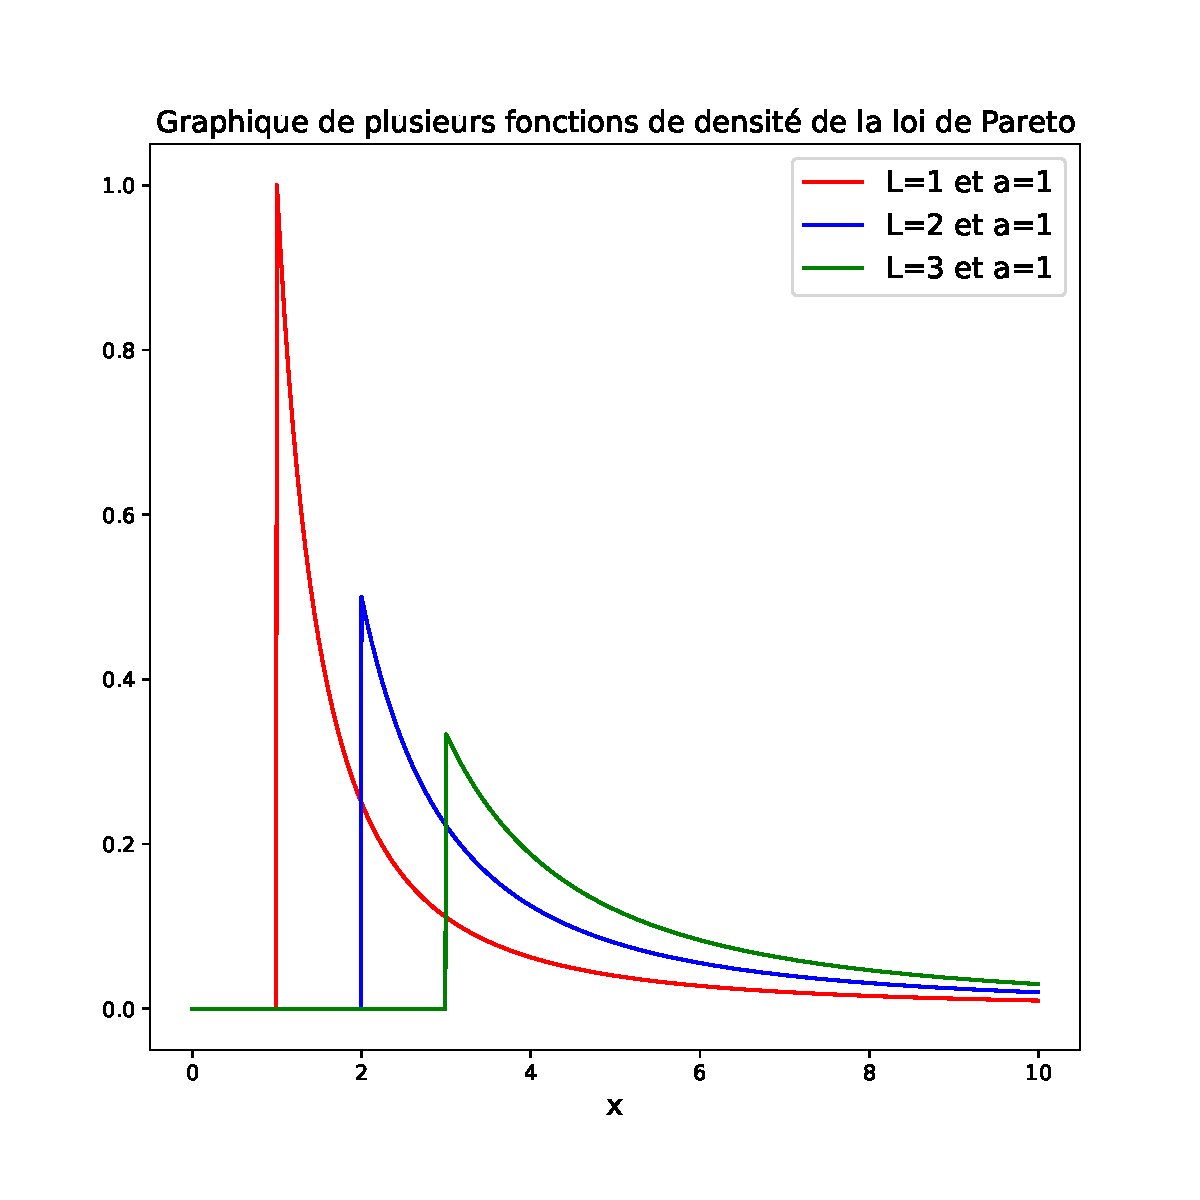
\includegraphics[scale=0.25]{graphiques_Pareto.pdf}

\end{column}

\pause
\begin{column}{0.5\linewidth}

\vspace*{2cm}
Remarque: particularité de la loi de Pareto, pour le cas $a=1$, on a que la mediane de la distribution est $2L.$

\end{column}

\end{columns}

\end{frame}

\begin{frame}

\frametitle{Les bandits de Pareto avec $a=1$}

À chaque pas de temps $t=1,2,\ldots,T,$ l'agent:

\begin{itemize}

\item[$\bullet$] Sélectionne une action $k_t\in\left\{1,2,\ldots,K\right\}$

\item[$\bullet$] Observe une reward $r_t\sim \mathrm{Pareto}(L_{k_t},1)$

\end{itemize}

\vfill
\pause

L'action optimale et la localisation optimale sont définis à partir de la localisation des différents bras:

\pause
$$\displaystyle L^{\star} := \max_k L_k \qquad \text{et} \qquad k^{\star} := \underset{k}{\mathrm{argmax}} L_k$$ 

\pause
\vfill

le gap (regret) associé à l'action $k$ devient $\Delta_k= L^{\star}-L_k$ 

\pause
\vfill

Mesure de performance empirique d'un agent: $\displaystyle R(T)=\sum_{t=1}^T \Delta_{k_t}$

\end{frame}

\begin{frame}
\frametitle{Estimateur de la localisation $L$ d'une loi de Pareto et résultats préliminaires}
Un estimateur naturel pour $L$ à partir d'un jeux de données $\mathcal{X}=\left\{X_1,X_2,X_3,\ldots,X_T\right\}$ tirées d'une loi $Pareto(L,1)$ est $\widehat{L}=\min(\mathcal{X})$ ou encore $\widehat{L}=\frac{1}{2}\mathrm{MED}(\mathcal{X})$

\pause
\vfill

On peut donc généraliser les algorithmes classiques comme \underline{$\epsilon$-greedy}, \underline{ETC}, \underline{Boltzmann/Softmax}
  
\pause
\vfill

Voici le résultat d'une expérience sur $N=200$ instances de bandits Pareto à deux bras avec $L_1, L_2\sim\mathcal{U}([0,1])$ et $a=1,$ où l'on a joué \underline{$\epsilon_t$-greedy} avec $\epsilon_t=1/\sqrt{t}$ sur un horizone de $T=1000$ pas de temps.

\vfill

\begin{center}
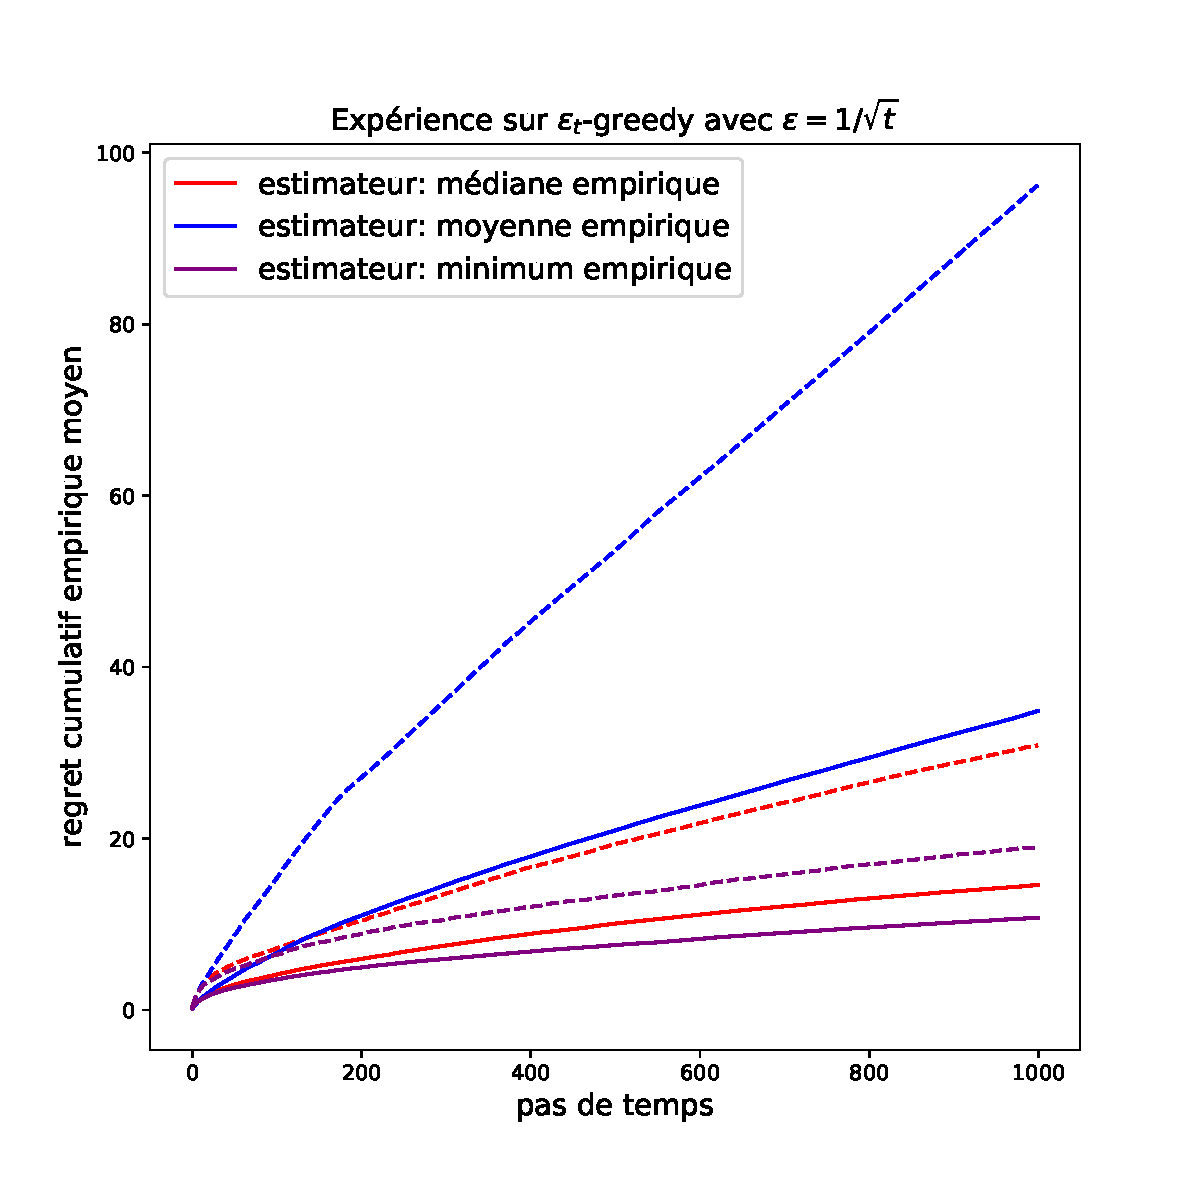
\includegraphics[scale=0.25]{exp-Pareto.pdf}
\end{center}

\end{frame}
                          
\begin{frame}

\frametitle{La suite }

\pause
\vfill

\begin{itemize}

\item[$\bullet$]
Modélisation d'un problème concret.

\begin{columns}[T] % align columns

\begin{column}{0.5\linewidth}
%\color{red}\rule{\linewidth}{4pt}
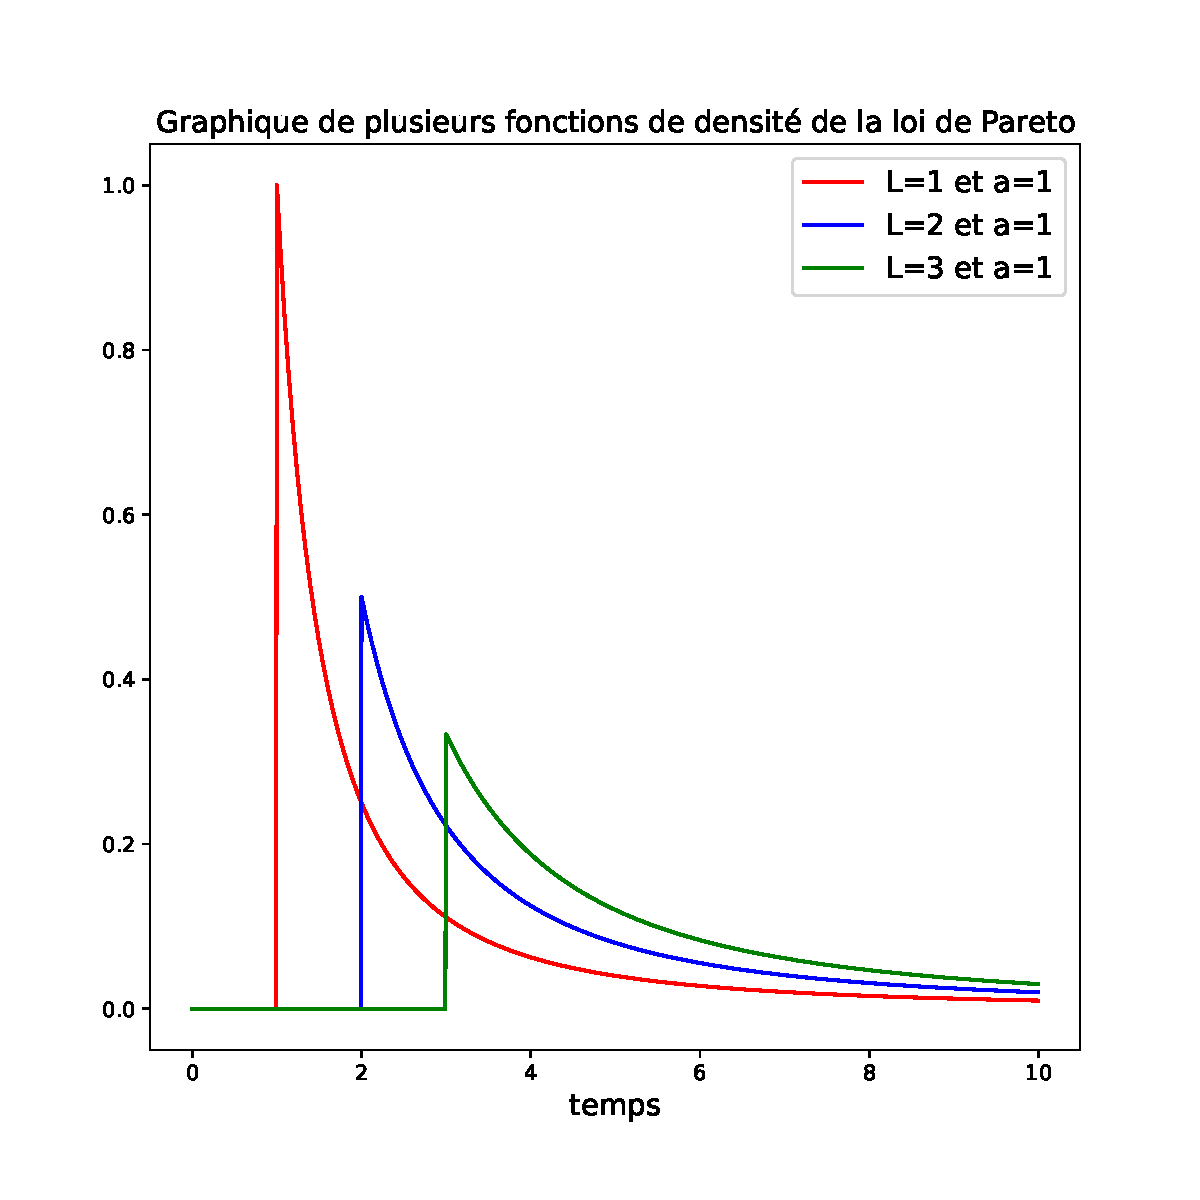
\includegraphics[scale=0.25]{graphiques_Pareto-temps.pdf}
\end{column}%

\hfill
\pause

\begin{column}{0.5\linewidth}
%\color{blue}\rule{\linewidth}{4pt}
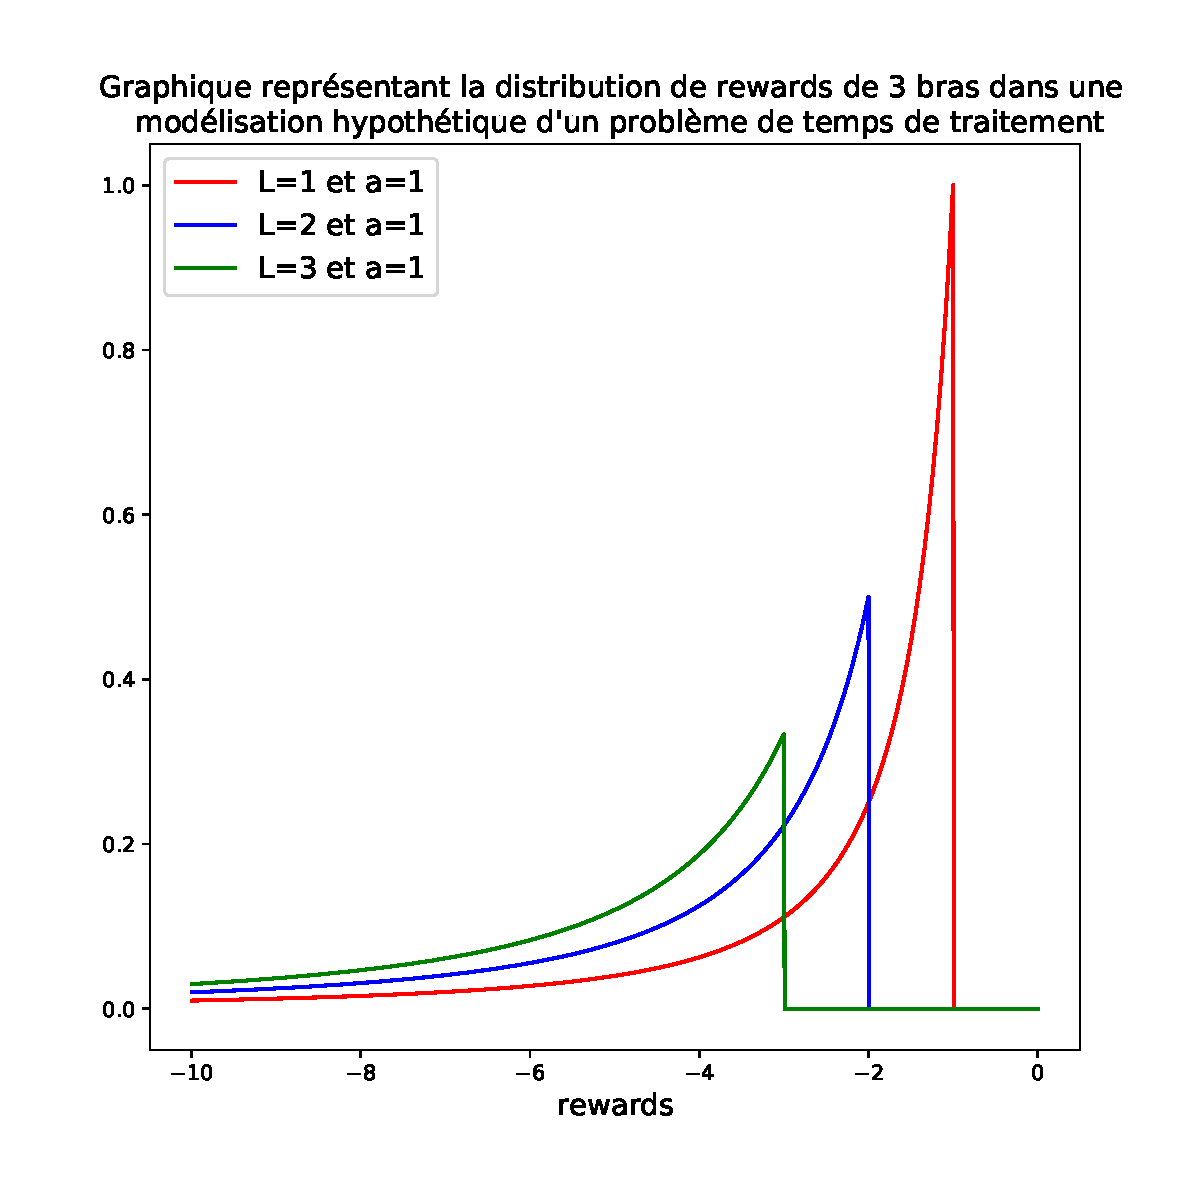
\includegraphics[scale=0.25]{graphiques_Pareto-inverse.pdf}
\end{column}%
\end{columns}

\pause
\vfill

\item[$\bullet$] Extension à des algorithmes plus complexes, par exemple les UCB, Thompson sampling, etc...\\

{\it S. Bubeck, N. Cesa-Bianchi and G. Lugosi, "Bandits With Heavy Tail," in IEEE Transactions on Information Theory, vol. 59, no. 11, pp. 7711-7717, Nov. 2013, doi: 10.1109/TIT.2013.2277869.}

\pause
\vfill

\item[$\bullet$] Généralisation du problème (définition de la mesure d'une performance générale qui ne dépend pas de la loi), possiblement basée sur des notions de dominance entre des variables aléatoires.

\end{itemize}

\end{frame}

\vfill

\end{document}
